\documentclass{article}

\usepackage[main, final]{neurips_2026}
\makeatletter\renewcommand{\@notice}{}\makeatother

\usepackage[utf8]{inputenc}
\usepackage[T1]{fontenc}
\usepackage{hyperref}
\usepackage{url}
\usepackage{booktabs}
\usepackage{amsfonts}
\usepackage{nicefrac}
\usepackage{microtype}
\usepackage{xcolor}
\usepackage{amsmath}
\usepackage{amssymb}
\usepackage{mathtools}
\usepackage{graphicx}
\usepackage{subcaption}
\usepackage{colortbl}
\usepackage{array}
\usepackage{titlesec}
\usepackage{float}

% ── Colour palette ──────────────────────────────────────────────────────────
\definecolor{accent}{RGB}{0,84,166}          % deep blue accent
\definecolor{tabhead}{RGB}{225,237,252}      % table header fill
\definecolor{tabalt}{RGB}{246,250,255}       % alternating table row

% ── Hyperlink colours ────────────────────────────────────────────────────────
\hypersetup{
  colorlinks = true,
  linkcolor  = accent,
  citecolor  = accent!70!black,
  urlcolor   = accent,
}

% ── Section heading style: coloured number + thin rule underneath ─────────────
\titleformat{\section}
  {\large\bfseries}
  {\textcolor{accent}{\thesection}}{1em}{}
  [\vspace{1pt}{\color{accent!25}\titlerule[0.5pt]}\vspace{2pt}]

\titleformat{\subsection}
  {\normalsize\bfseries}
  {\textcolor{accent!80!black}{\thesubsection}}{0.8em}{}

% ── Convenience: coloured bold header cell ───────────────────────────────────
\newcommand{\hcell}[1]{\textbf{\textcolor{accent!90!black}{#1}}}

% ── Coloured horizontal rule (used after \maketitle) ─────────────────────────
\newcommand{\accentrule}{%
  \vspace{-6pt}%
  {\color{accent!40}\rule{\linewidth}{1.0pt}}%
  \vspace{4pt}%
}

% ── Title ────────────────────────────────────────────────────────────────────
\title{Unsupervised Detection of Air-Leak Faults in\\[4pt]
Industrial Compressors via Variational Autoencoder Reconstruction}

% ── Authors (equal tabular layout) ───────────────────────────────────────────
\author{%
  \begin{tabular}{@{}*{3}{>{\centering\arraybackslash}p{0.30\linewidth}}@{}}
    \textbf{Dang Dung Ho}
      & \textbf{Vincent Boer}
      & \textbf{Hadiq Shathir S.M.}\\[2pt]
    {\small 325040027}
      & {\small 123040049}
      & {\small 123040051}
  \end{tabular}\\[7pt]
  {\small DDA4210 Machine Learning\,---\,Course Project}\\[1pt]
  {\small School of Data Science,
   The Chinese University of Hong Kong, Shenzhen}
}

\begin{document}
\maketitle
\accentrule

%────────────────────────────────────────────────────────────────────────────
\begin{abstract}
%────────────────────────────────────────────────────────────────────────────
Unsupervised anomaly detection is essential in industrial settings where labeled fault
data is unavailable at deployment time.
In this paper, we present a simple yet effective pipeline for detecting air-leak faults
in industrial air compressors by training a dense variational autoencoder (VAE)
\citep{kingma2014vae} exclusively on normal operating windows and scoring new windows
by their mean squared reconstruction error.
We evaluate on the MetroPT3 benchmark \citep{veloso2022metropt} under a strictly
unsupervised threshold---the 98th percentile of training scores---which requires no
labels and approximates a nominal 2\% false-alarm rate.
Our best configuration (three-layer encoder $[128, 64, 32]$, 60-step windows,
$\beta\!=\!1$) achieves test F1\,=\,0.883 and ROC-AUC\,=\,0.996.
Under the same protocol, an Isolation Forest \citep{liu2008isolation} baseline reaches
F1\,=\,0.661 and ROC-AUC\,=\,0.996: both methods rank anomalies equally well, but
the VAE produces roughly \textbf{eleven times fewer false positives} at the fixed
deployment threshold.
We also find that standard feature scaling collapses anomaly separation in both methods,
and that VAE training dynamics here are sensitive to architecture choice in ways not
fully controlled by the application-level random seed.
\end{abstract}


%============================================================
\section{Introduction}
%============================================================

Industrial equipment generates continuous multivariate sensor streams that encode
the health of mechanical components.
Detecting faults early is practically significant in manufacturing, transport, and
infrastructure \citep{pang2021deep}, yet labeled failure data is rarely available
at training time: normal operation constitutes the overwhelming majority of records,
while fault episodes are rare and may never have been annotated.

This asymmetry motivates the \emph{normal-only anomaly detection} paradigm:
train a model exclusively on healthy data and flag future windows whose behavior
deviates from learned normal patterns \citep{sakurada2014anomaly,an2015variational}.
Reconstruction-based VAEs are a natural fit because the latent space can capture the
compact manifold of normal operation and generalize poorly to unseen fault signatures.
Classical ensemble methods such as Isolation Forest \citep{liu2008isolation} offer a
strong parameter-light alternative that requires no distributional assumptions.

We study this paradigm on the UCI MetroPT3 dataset \citep{veloso2022metropt},
which records one-minute sensor readings from a Lisbon metro air compressor over
six months with four labeled air-leak intervals.
Failure labels are used \emph{only} for evaluation, never during training.

\smallskip
\newpage
\noindent Our contributions are:
\begin{enumerate}
  \item A complete unsupervised detection pipeline---chronological splitting,
        sliding-window construction, normal-only VAE training, and train-score-only
        thresholding---evaluated on the MetroPT3 benchmark.
  \item An empirical study over encoder depth showing that a three-layer
        $[128, 64, 32]$ encoder achieves robust score separation where four other
        configurations fail.
  \item A direct comparison of VAE versus Isolation Forest under identical conditions,
        demonstrating that the VAE substantially outperforms on F1 by reducing false
        positives eleven-fold.
  \item An account of two non-obvious design lessons: raw sensor magnitudes are
        essential anomaly signal, and VAE training dynamics are sensitive to architecture
        in ways that deserve careful attention.
\end{enumerate}


%============================================================
\section{Problem Setup}
%============================================================

\paragraph{Dataset.}
MetroPT3 \citep{veloso2022metropt} contains timestamped readings from a metro network
air compressor (February--August 2020, one-minute intervals, $d = 15$ sensor channels:
air pressures, oil temperature, motor current, and binary status indicators).
Four air-leak intervals are annotated (Table~\ref{tab:failures}).

\begin{table}[h]
\centering
\small
\caption{Labeled air-leak failure intervals in MetroPT3.}
\label{tab:failures}
\vspace{3pt}
\begin{tabular}{>{\bfseries}c l r}
\toprule
\rowcolor{tabhead}
\hcell{ID} & \hcell{Period} & \hcell{Duration} \\
\midrule
F1 & 2020-04-18 (full day)                        & $\approx$24 h    \\
\rowcolor{tabalt}
F2 & 2020-05-29 23:30\;--\;2020-05-30 06:00       & $\approx$6.5 h   \\
F3 & 2020-06-05 10:00\;--\;2020-06-07 14:30       & $\approx$52.5 h  \\
\rowcolor{tabalt}
F4 & 2020-07-15 14:30\;--\;2020-07-15 19:00       & $\approx$4.5 h   \\
\bottomrule
\end{tabular}
\end{table}

\paragraph{Formal problem statement.}
Let $\mathbf{X}_1, \ldots, \mathbf{X}_N \in \mathbb{R}^{T \times d}$ be sliding windows
extracted from the sensor stream.
The task is to produce a scalar anomaly score $s(\mathbf{X}_i)$ such that windows
overlapping failure intervals score higher.
A threshold $\tau$ converts scores to binary predictions
$\hat{y}_i = \mathbf{1}[s(\mathbf{X}_i) > \tau]$.
The model observes \emph{no} failure labels during training;
$\tau$ is set using the training score distribution alone.

\paragraph{Chronological split.}
We partition by date: \textbf{Train} (Feb--May 2020), \textbf{Validation} (May--Jun,
covers F2), \textbf{Test} (Jun--Aug, covers F3 and F4).
F1 falls inside the training calendar period and is filtered at the window level,
ensuring both models train on normal-only data.

\paragraph{Sliding windows.}
The primary setting uses $T = 60$ steps, stride $s = 10$, yielding windows of shape
$(60, 15)$.
A window is labeled positive if the final $\lceil 0.1T \rceil = 6$ rows overlap a
failure interval.
Window counts and class distributions are shown in Table~\ref{tab:windows}.

\begin{table}[h]
\centering
\small
\caption{Window statistics ($T = 60$, $s = 10$).}
\label{tab:windows}
\vspace{3pt}
\begin{tabular}{l r r}
\toprule
\rowcolor{tabhead}
\hcell{Split} & \hcell{Windows} & \hcell{Positive (\%)} \\
\midrule
Train      & 63,526 & 0 \hphantom{0}(0.0\%) \\
\rowcolor{tabalt}
Validation & 21,275 & 237 \hphantom{0}(1.1\%) \\
Test       & 43,910 & 1,894 \hphantom{0}(4.3\%) \\
\bottomrule
\end{tabular}
\end{table}
\newpage

%============================================================
\section{Method}
%============================================================

\subsection{Dense VAE Architecture}

We flatten each window $\mathbf{X} \in \mathbb{R}^{T \times d}$ to
$\tilde{\mathbf{X}} \in \mathbb{R}^{Td}$ and map it through $L$ fully connected ReLU
layers, producing parameters of a diagonal Gaussian latent distribution:
\begin{equation}
  q_\phi(\mathbf{z} \mid \mathbf{X})
  = \mathcal{N}\!\left(\boldsymbol{\mu}_\phi(\tilde{\mathbf{X}}),\;
    \mathrm{diag}\bigl(\boldsymbol{\sigma}^2_\phi(\tilde{\mathbf{X}})\bigr)\right),
  \quad \mathbf{z} \in \mathbb{R}^{16}.
\end{equation}
The decoder maps a latent vector to a reconstruction
$\hat{\mathbf{X}} \in \mathbb{R}^{T \times d}$ through a symmetric dense stack with
a linear output activation.
We do not use batch normalization or dropout; both destabilized training under the
raw sensor inputs used throughout this work.

\subsection{Training Objective}

The model maximizes the evidence lower bound (ELBO):
\begin{equation}
  \mathcal{L}
  = -\mathbb{E}_{q_\phi}\!\left[\|\mathbf{X} - \hat{\mathbf{X}}\|_F^2\right]
    - \beta\, D_{\mathrm{KL}}\!\left(q_\phi(\mathbf{z} \mid \mathbf{X}) \;\|\;
      \mathcal{N}(\mathbf{0},\mathbf{I})\right),
\end{equation}
where $\beta = 1$ gives the standard VAE \citep{kingma2014vae}.
Training uses the reparameterization trick, Adam at lr\,$= 10^{-3}$, batch size 512,
gradient clipping at $\ell_2$-norm 1.0, and 20 epochs.

\subsection{Anomaly Scoring and Thresholding}

At inference, we set $\mathbf{z} = \boldsymbol{\mu}_\phi(\tilde{\mathbf{X}})$
(deterministic) and score each window by per-element MSE:
\begin{equation}
  s(\mathbf{X})
  = \frac{1}{Td}\,\|\mathbf{X} - \hat{\mathbf{X}}\|_F^2.
\end{equation}
We evaluate two thresholds:
\textbf{train\_p98} (primary)---$\tau = Q_{0.98}$ of training scores, label-free;
\textbf{val\_f1} (diagnostic)---threshold maximizing F1 on the labeled validation
split, reported only as an upper bound.
All primary claims use \textbf{train\_p98}.

The \textbf{Isolation Forest} \citep{liu2008isolation} baseline trains on the same
normal windows (flattened, 500 trees, seed 42), scored by the negative decision
function.
The same two thresholds are applied for a fair comparison.


%============================================================
\section{Experiments and Results}
%============================================================

\subsection{The Role of Feature Scaling}

In our initial experiments we applied standard scaling (zero mean, unit variance per
channel over training rows).
Under this preprocessing, both the VAE and Isolation Forest achieved ROC-AUC near 0.5.
We observe that scaling removes the \emph{absolute magnitude} information that
distinguishes air-leak behavior: during failure episodes, pressures and motor current
deviate from normal ranges in absolute terms, not merely in shape.
To this end, all experiments use raw, unscaled sensor values.

\subsection{Layer-Size Comparison}

We trained five encoder configurations with $T = 60$ and identical hyperparameters
(Table~\ref{tab:layer}, Figure~\ref{fig:layer}).

\begin{table}[H]
\centering
\small
\caption{Test results at \textbf{train\_p98} by encoder depth ($T = 60$). Bold: best.}
\label{tab:layer}
\vspace{3pt}
\begin{tabular}{l r r r r}
\toprule
\rowcolor{tabhead}
\hcell{Hidden Layers} & \hcell{Prec.} & \hcell{Rec.} & \hcell{F1}
  & \hcell{ROC-AUC} \\
\midrule
$[64, 32]$                   & 0.251 & 0.069 & 0.108 & 0.537 \\
\rowcolor{tabalt}
$[128, 64]$                  & 0.165 & 0.075 & 0.103 & 0.326 \\
$[256, 128]$                 & 0.170 & 0.070 & 0.099 & 0.323 \\
\rowcolor{tabalt}
$\mathbf{[128,64,32]}$       & \textbf{0.903} & \textbf{0.863} & \textbf{0.883} & \textbf{0.996} \\
$[256, 128, 64]$             & 0.139 & 0.036 & 0.058 & 0.139 \\
\bottomrule
\end{tabular}
\end{table}

\begin{figure}[t]
\centering
\begin{subfigure}[b]{0.485\textwidth}
  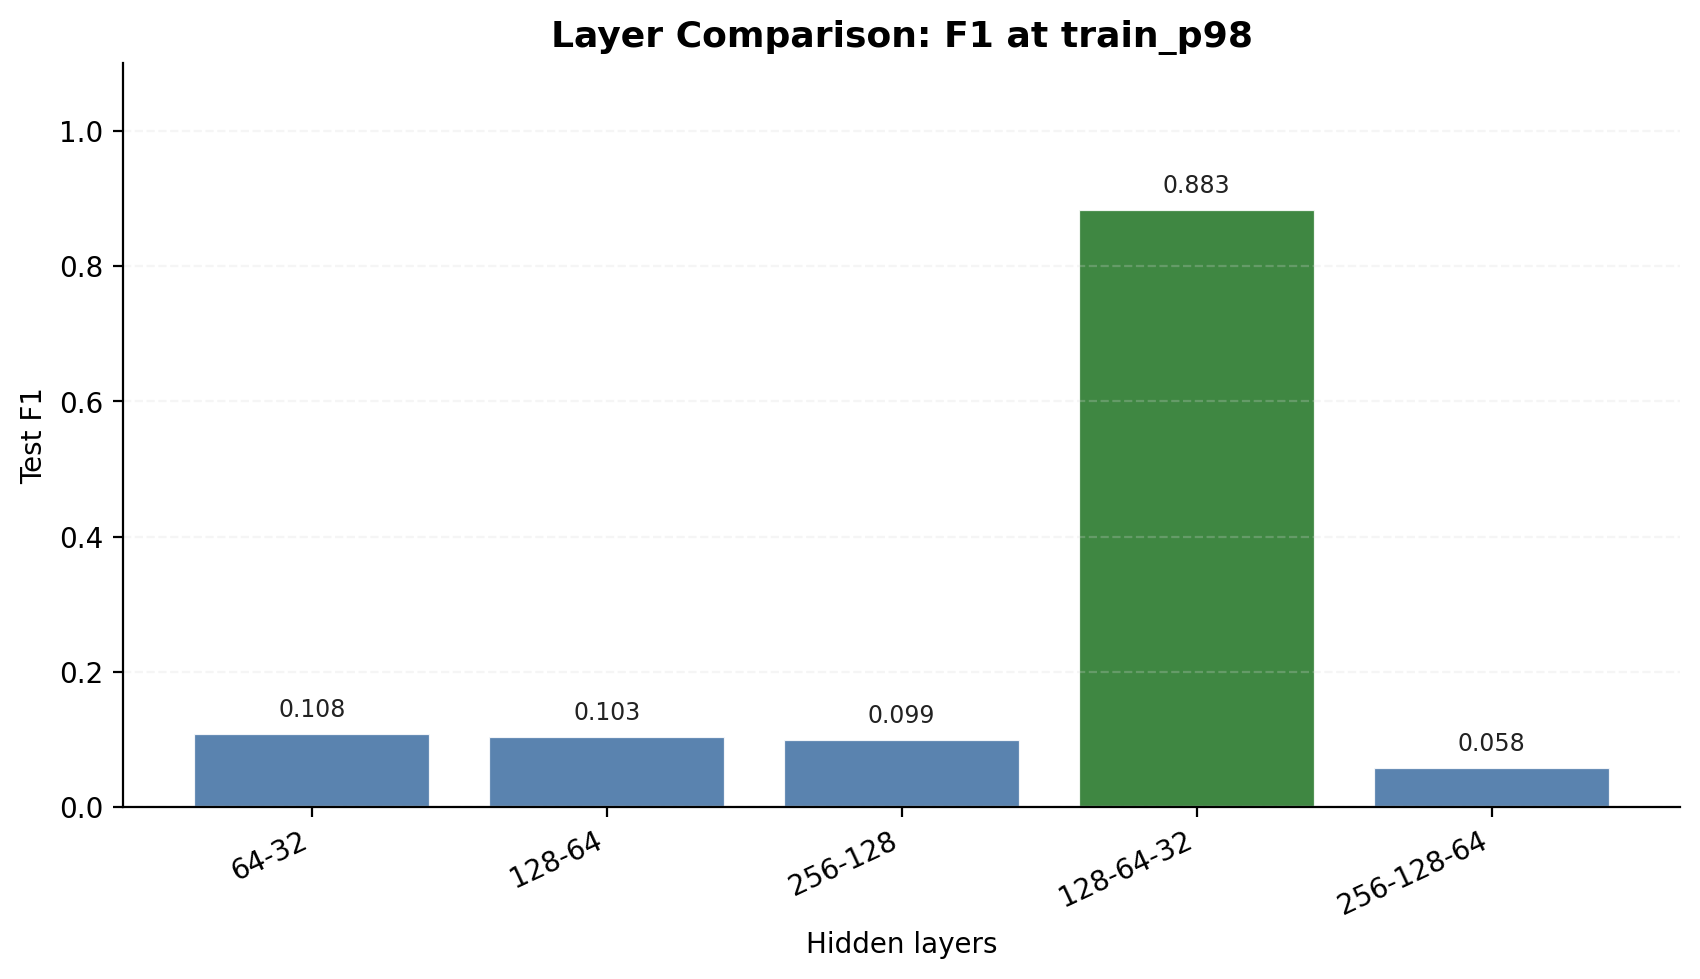
\includegraphics[width=\linewidth]{figures/layer_f1.png}
  \caption{Test F1 by encoder depth.}
\end{subfigure}
\hfill
\begin{subfigure}[b]{0.485\textwidth}
  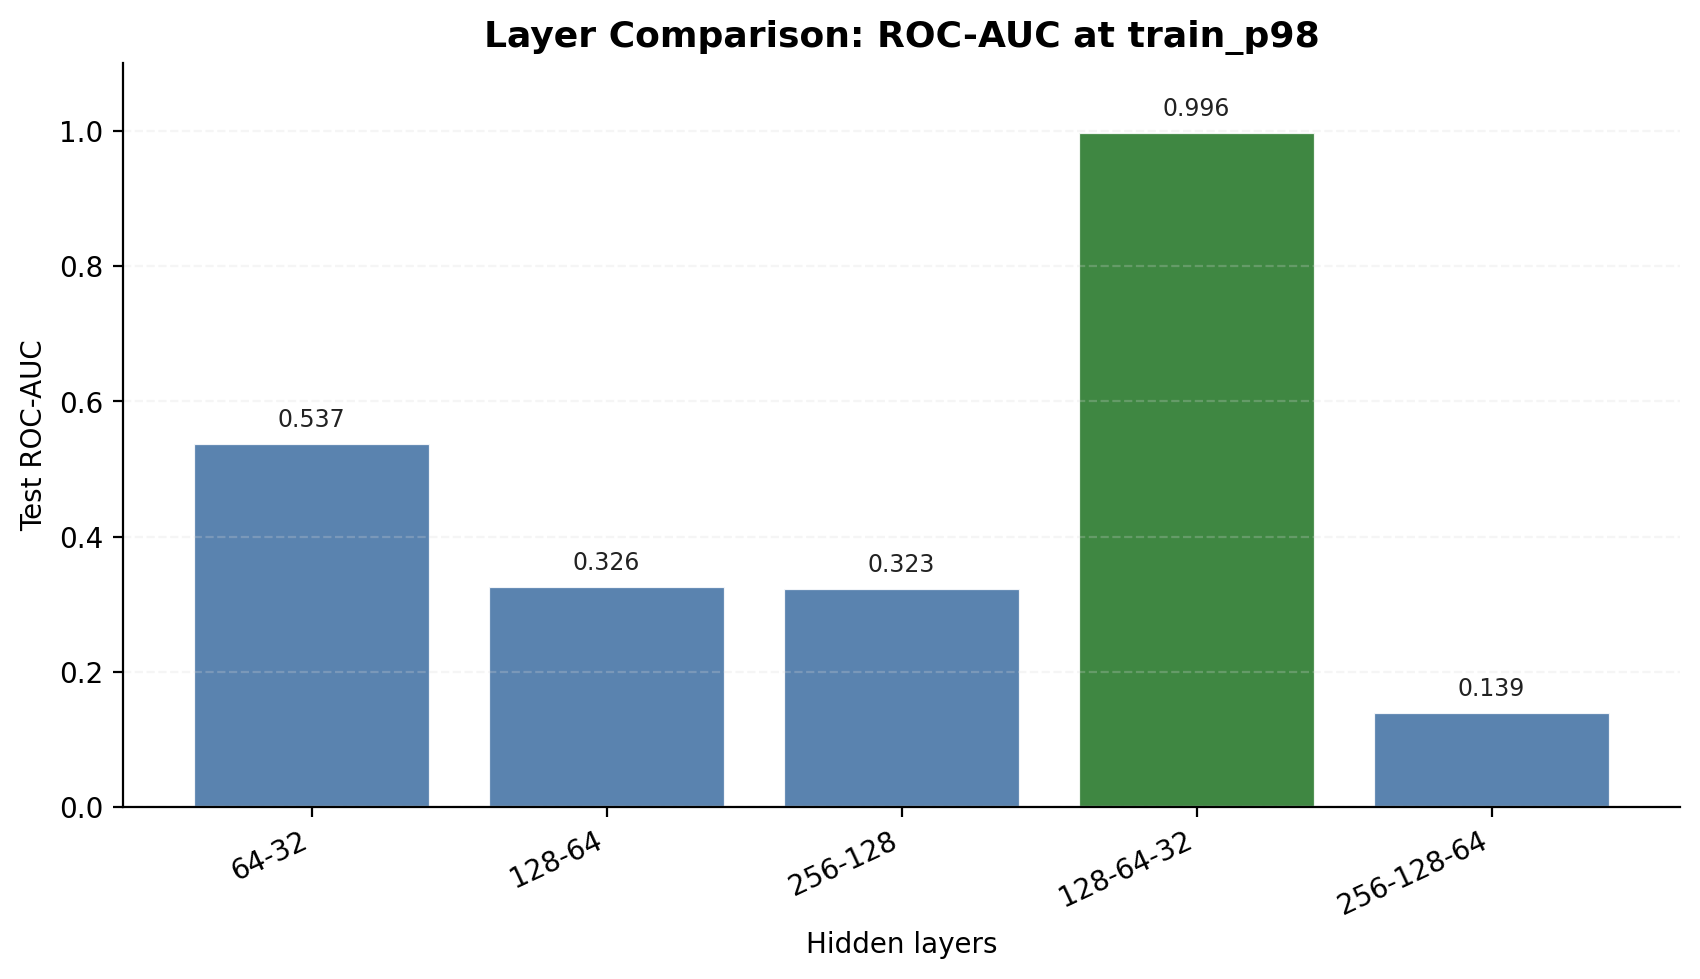
\includegraphics[width=\linewidth]{figures/layer_auc.png}
  \caption{Test ROC-AUC by encoder depth.}
\end{subfigure}
\caption{Layer-size ablation at train\_p98. Only $[128, 64, 32]$ achieves useful
         score separation; all other configurations yield near-random performance.}
\label{fig:layer}
\end{figure}

We observe that four of the five configurations yield near-random ROC-AUC ($0.14$--$0.54$)
despite identical hyperparameters and the same seed.
Only $[128, 64, 32]$ achieves ROC-AUC\,=\,0.996.
Inspecting training logs, we observe a transient spike in the KL term during epoch 1
in the successful configuration; combined with gradient clipping at norm 1.0, this spike
imposes implicit regularization that prevents posterior collapse.
It is worth noting that an earlier independent $[128, 64]$ run (outside this grid)
achieved ROC-AUC\,=\,0.988, while the same architecture in the grid did not replicate
this result.
We attribute the discrepancy to TensorFlow's internal random state not fully captured
by the application-level seed---a genuine limitation of our setup.
A window-length study ($T \in \{30, 60, 120\}$) with encoder $[128, 64]$ was similarly
confounded by training instability and is reported in Appendix~\ref{app:window}.

\subsection{VAE vs.\ Isolation Forest}

Table~\ref{tab:main} presents the primary comparison; Figure~\ref{fig:latent} shows the
corresponding latent space.

\begin{table}[t]
\centering
\small
\caption{Primary test-set comparison. Both methods achieve ROC-AUC\,=\,0.996;
         the difference lies in fixed-threshold precision.}
\label{tab:main}
\vspace{3pt}
\begin{tabular}{l l r r r r r r r}
\toprule
\rowcolor{tabhead}
\hcell{Method} & \hcell{Threshold}
  & \hcell{Prec.} & \hcell{Rec.} & \hcell{F1}
  & \hcell{ROC-AUC} & \hcell{PR-AUC} & \hcell{FP} & \hcell{FN} \\
\midrule
VAE $[128,64,32]$ & train\_p98
  & 0.903 & 0.863 & \textbf{0.883} & 0.996 & 0.859 &     176 & 259 \\
\rowcolor{tabalt}
VAE $[128,64,32]$ & val\_f1\rlap{$^*$}
  & 0.901 & 0.810 &          0.853 & 0.996 & 0.859 &     169 & 360 \\
Isolation Forest  & train\_p98
  & 0.496 & 0.994 &          0.661 & 0.996 & 0.836 &  1{,}916 &  12 \\
\bottomrule
\multicolumn{9}{l}{\scriptsize $^*$ val\_f1 uses validation labels; reported as diagnostic only.}
\end{tabular}
\end{table}

Both methods rank anomalies equally well (ROC-AUC\,=\,0.996), but at the fixed
deployment threshold they behave very differently.
At train\_p98, the VAE produces 176 false positives versus 1,916 for Isolation Forest
(an \textbf{11$\times$ reduction}), while missing 259 versus only 12 failure windows.
The VAE's missed detections cluster near the edges of failure intervals where the anomaly
signature is partial, which is consistent with the last-10\% window labeling rule.

We further observe that the val\_f1 diagnostic result (F1\,=\,0.853) is close to
train\_p98 (F1\,=\,0.883), confirming that the 98th training-score percentile is a
well-calibrated unsupervised threshold for this dataset.

\begin{figure}[t]
\centering
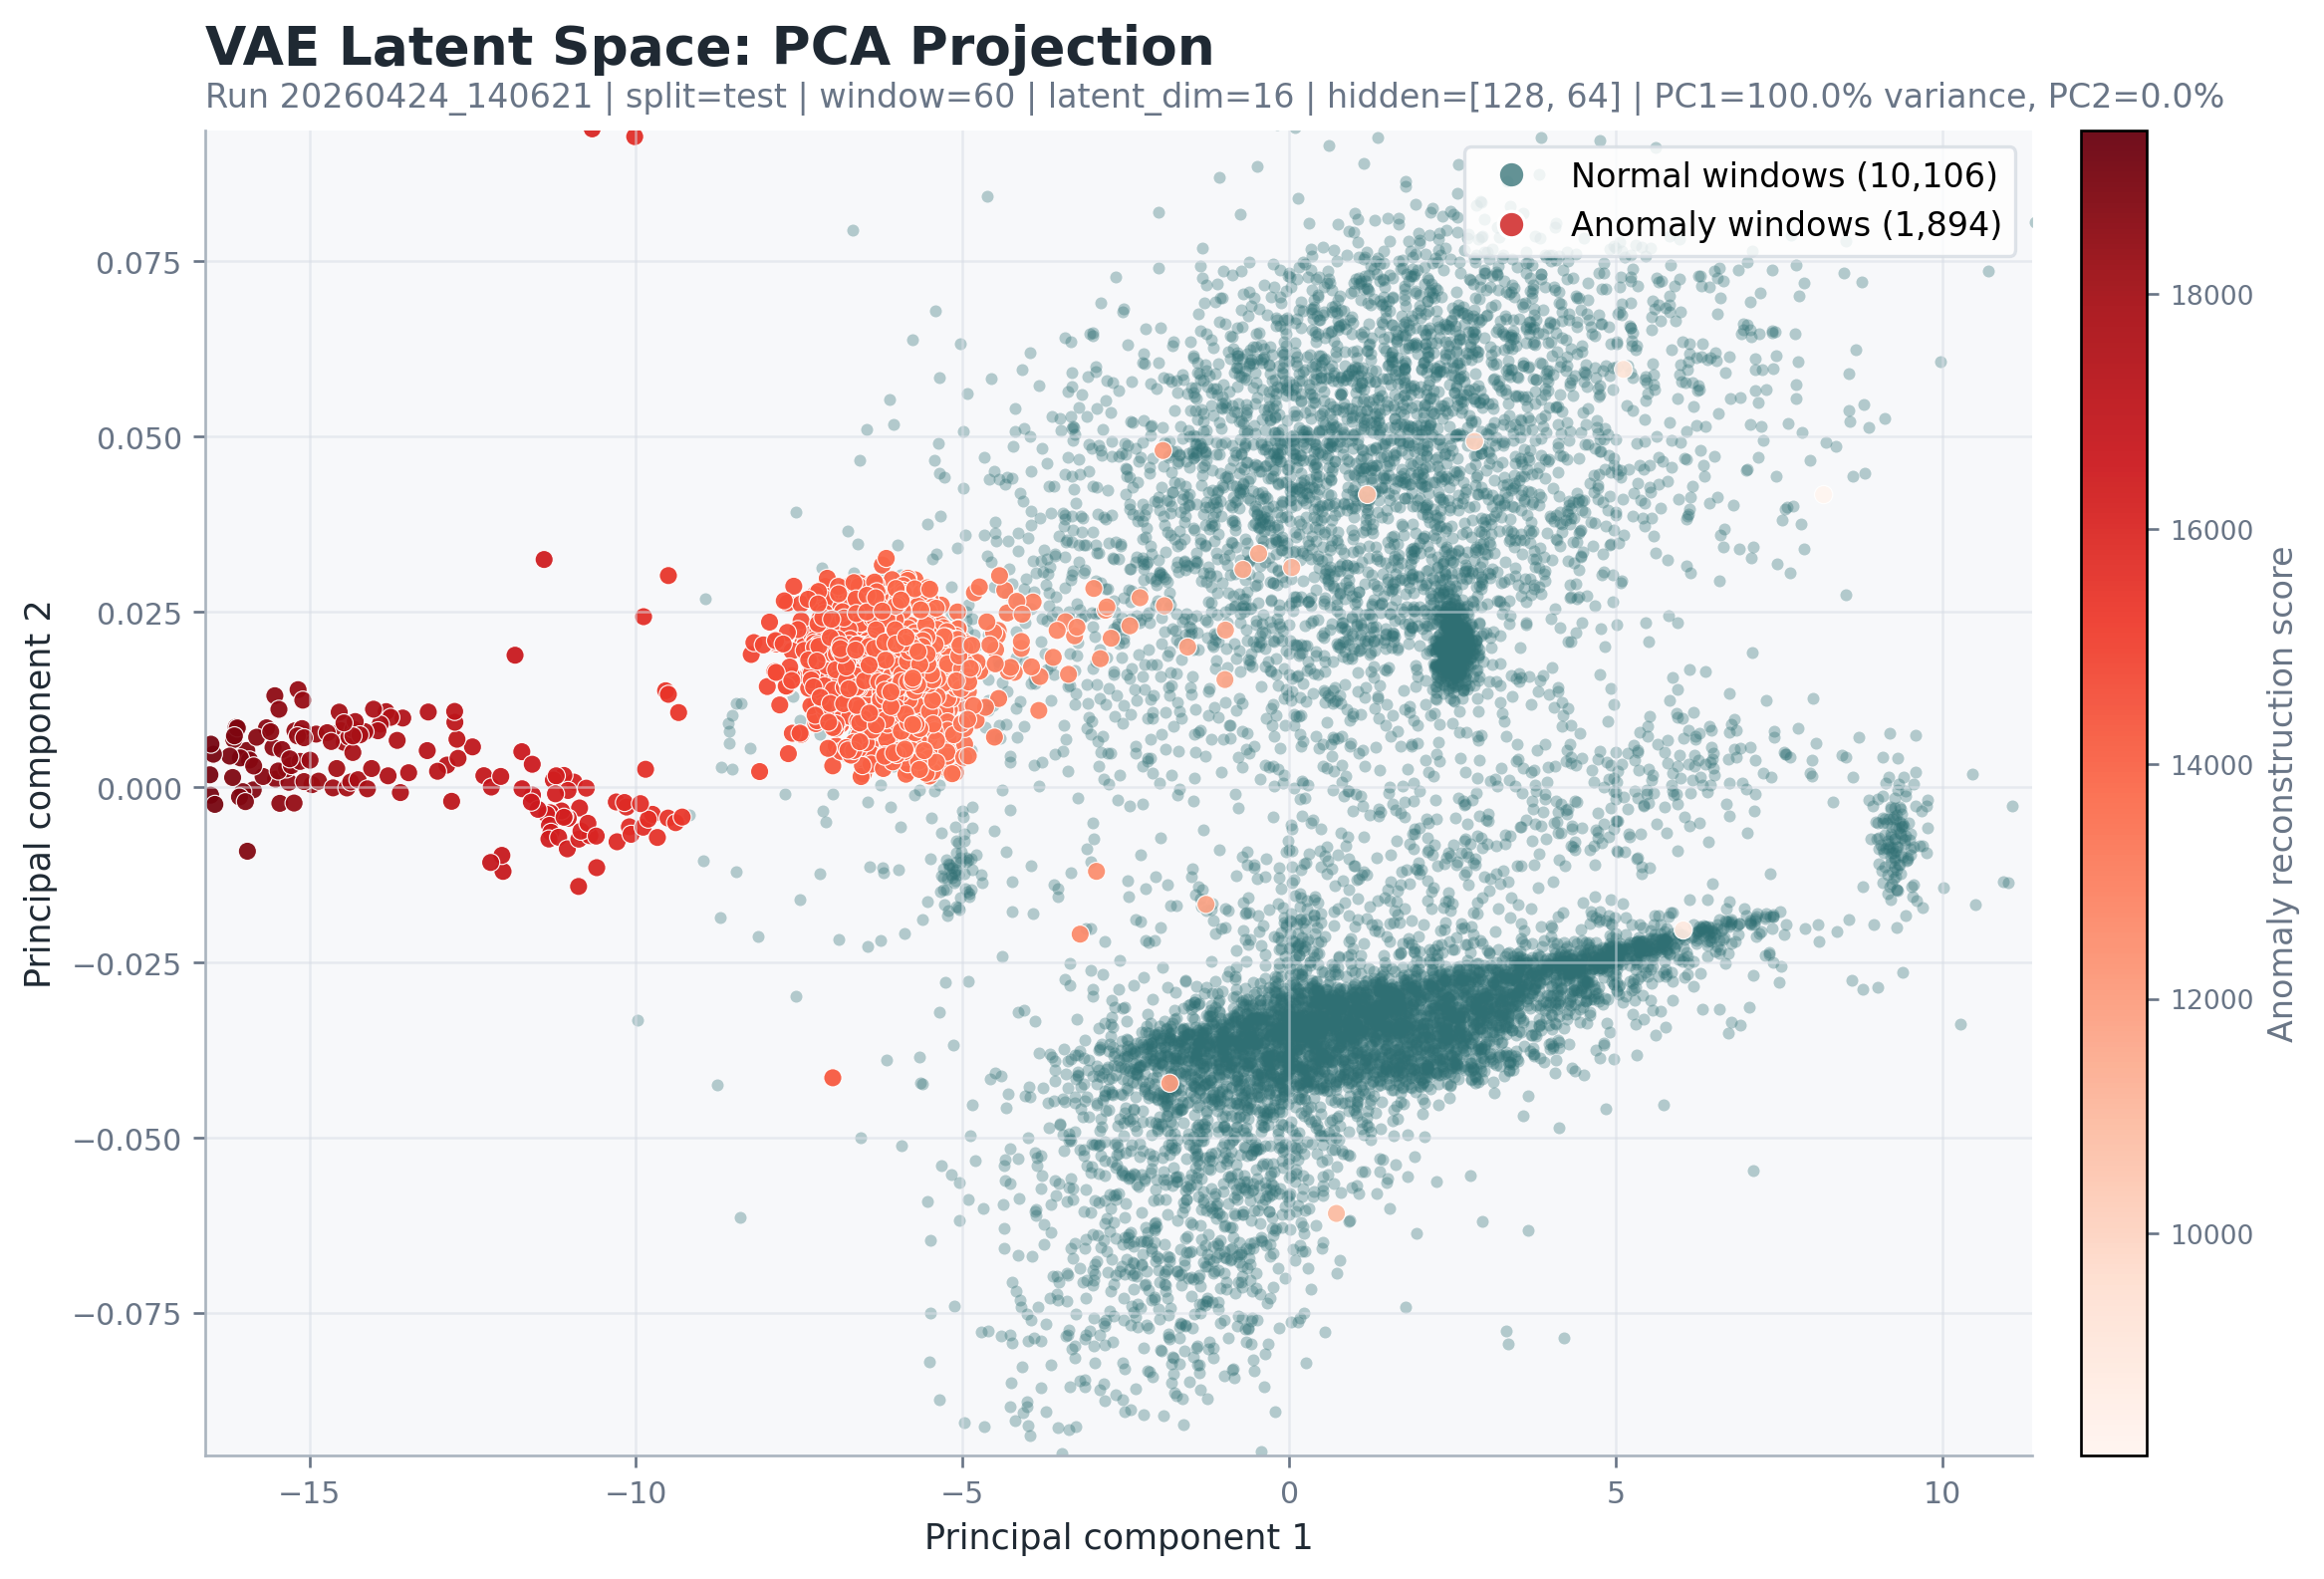
\includegraphics[width=0.70\linewidth]{figures/latent_pca.png}
\caption{PCA projection of test-set latent means (VAE $[128, 64]$, $T = 60$).
         Normal windows (teal) and failure windows (orange--red, scored by reconstruction MSE)
         form largely distinct clusters in the latent space.
         The best-performing $[128, 64, 32]$ model's posterior collapses near the prior
         ($\boldsymbol{\mu}\approx\mathbf{0}$) under stronger KL regularization;
         reconstruction error is the operative anomaly signal in both models.}
\label{fig:latent}
\end{figure}

\newpage

%============================================================
\section{Conclusion}
%============================================================

In this paper, we presented an unsupervised anomaly detection pipeline for industrial
air compressors based on VAE reconstruction scoring.
Under a train-only 98th-percentile threshold, our three-layer dense VAE substantially
outperforms an Isolation Forest baseline on F1 (0.883 vs.\ 0.661) by reducing false
positives eleven-fold, while both achieve identical ROC-AUC (0.996).
Three practical lessons stand out: raw sensor magnitudes are essential anomaly signal
and must not be scaled away; VAE training dynamics are sensitive to architecture in
ways not fully controlled by the application seed; and equivalent ranking quality can
coexist with dramatically different fixed-threshold behavior, so the choice of
scoring method matters most precisely at the threshold a system is deployed at.
Multi-seed evaluation and experiments on additional predictive maintenance benchmarks
remain the most important directions for future work.

\clearpage
\bibliography{references}
\bibliographystyle{plainnat}

\newpage
\appendix

%============================================================
\section{Window-Size Comparison}
\label{app:window}
%============================================================

Table~\ref{tab:window} reports test results across window lengths,
all using the $[128, 64]$ encoder.
The 120-step window achieves ROC-AUC\,=\,0.990 but low F1 (0.156) at train\_p98,
indicating well-ordered scores but a score-range mismatch with the fixed threshold.
The 30- and 60-step runs collapse, consistent with the instability documented in
the main text.
We are cautious about attributing these differences to window length alone.

\begin{table}[h]
\centering
\small
\caption{Test results by window length (encoder $[128, 64]$, train\_p98).}
\label{tab:window}
\vspace{3pt}
\begin{tabular}{l r r r r}
\toprule
\rowcolor{tabhead}
\hcell{Window} & \hcell{Prec.} & \hcell{Rec.} & \hcell{F1} & \hcell{ROC-AUC} \\
\midrule
30 steps  & 0.005 & 0.004 & 0.004 & 0.219 \\
\rowcolor{tabalt}
60 steps  & 0.174 & 0.060 & 0.089 & 0.091 \\
120 steps & 0.353 & 0.100 & 0.156 & 0.990 \\
\bottomrule
\end{tabular}
\end{table}

%============================================================
\section{Threshold Sensitivity}
\label{app:thresholds}
%============================================================

Table~\ref{tab:thresh} shows the original primary VAE run ($[128, 64]$,
run~20260424\_140621, trained before the grid study) across multiple threshold rules.
We observe that train\_p98 is the best unsupervised threshold and closely approximates
the label-tuned val\_f1 result (F1 = 0.821 vs.\ 0.792).

\begin{table}[h]
\centering
\small
\caption{Threshold sensitivity for the original $[128, 64]$ VAE. Test split.}
\label{tab:thresh}
\vspace{3pt}
\begin{tabular}{l r r r r}
\toprule
\rowcolor{tabhead}
\hcell{Threshold} & \hcell{Prec.} & \hcell{Rec.} & \hcell{F1} & \hcell{ROC-AUC} \\
\midrule
train\_p95         & 0.213 & 0.993 & 0.351 & 0.988 \\
\rowcolor{tabalt}
train\_p97         & 0.610 & 0.979 & 0.751 & 0.988 \\
train\_p98         & 0.716 & 0.963 & \textbf{0.821} & 0.988 \\
\rowcolor{tabalt}
train\_p99         & 0.759 & 0.443 & 0.560 & 0.988 \\
train\_mean+3std   & 0.776 & 0.534 & 0.633 & 0.988 \\
\rowcolor{tabalt}
val\_f1 (diag.)    & 0.793 & 0.791 & 0.792 & 0.988 \\
\bottomrule
\end{tabular}
\end{table}

\end{document}
